\documentclass{article} % For LaTeX2e
\usepackage{cos424,times}
\usepackage{hyperref}
\usepackage{url}
\usepackage{float}
\usepackage{graphicx}


\title{Music Genre Classification}


\author{
Abhinav Khanna\\
Student Researcher\\
\texttt{akhanna@princeton.edu} \\
\And
Amandeep Singh \\
Student Researcher \\
\texttt{email@princeton.edu} \\
}

\newcommand{\fix}{\marginpar{FIX}}
\newcommand{\new}{\marginpar{NEW}}

\begin{document}

\maketitle

\begin{abstract}
\end{abstract}

\section{Introduction}


\section{Related Work}


\section{Methods}
\subsection{Description of data}
The training data used in this paper comes from a set of 33 reference samples that have their entire genome bisulfite sequence. We primarily focus on the data for chromosome 1 for our analysis. The data consists of 33 reference samples with their methlyation proportions for each CpG site on the chromosome. We utilize this information to impute the values for the missing methlyation values in the test chromosome sample.

To better understand the relationships between different tissues, we computed the Pearson R correlation coefficient (Figure 2). Certain tissues have a meaningful, non-pure chance, correlation with other tissues suggesting that certain tissues may be more apt at predicting given test values than other tissues. We also know from Figure 1 that locations that are closer together have higher correlations, and are more similar to each other than locations that are further apart on the chromosome.

\begin{figure}[!ht]
\begin{center}
\caption{Pearson R Correlation for neighboring index locations}
\begin{minipage}[b]{0.40\linewidth}
	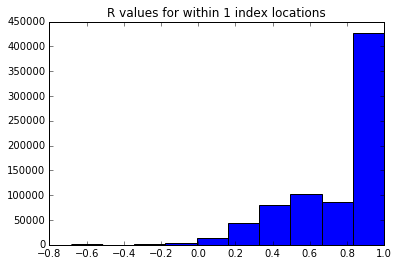
\includegraphics[scale=0.40]{CorrelationByLocation.png}
\end{minipage}
\quad
\end{center}
\end{figure}

\begin{figure}[!ht]
\begin{center}
\caption{Table of Correlation Values for Different Tissues}
\begin{minipage}[b]{0.40\linewidth}
	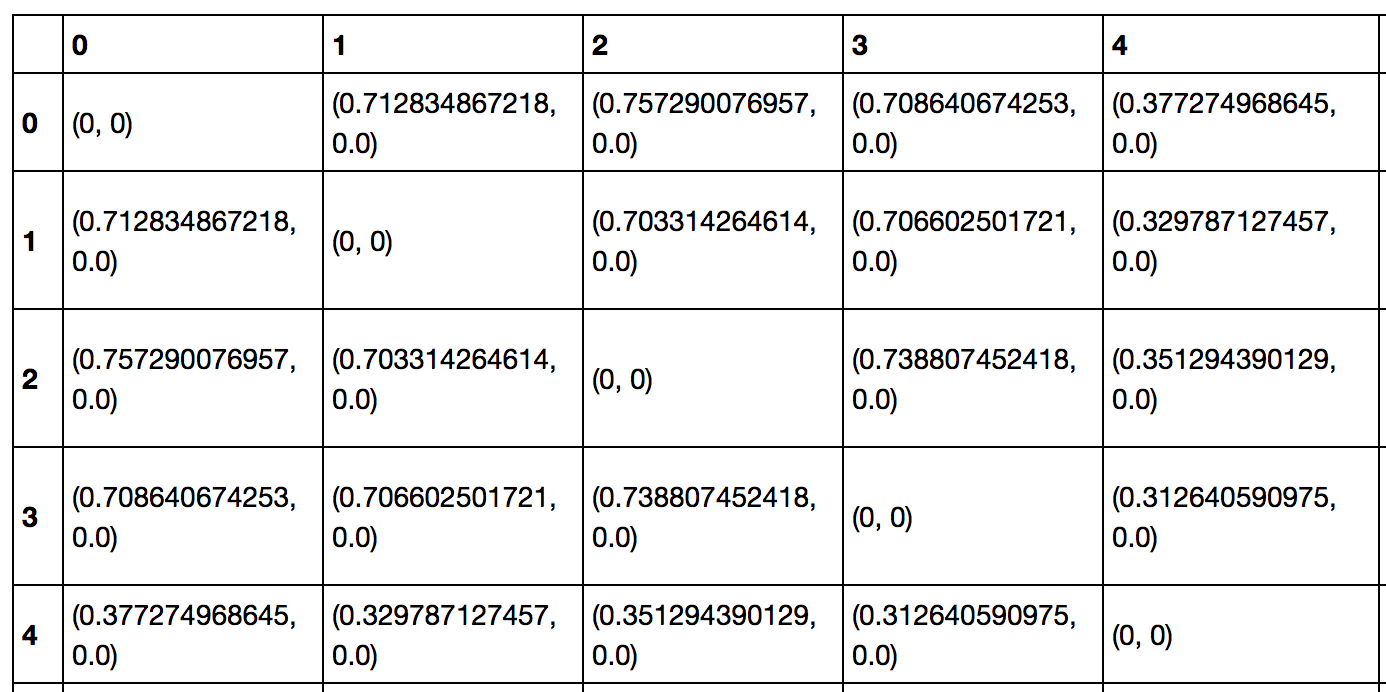
\includegraphics[scale=0.3]{table1.png}
\end{minipage}
\end{center}
\end{figure}

Examining the distribution of the mean methylation values across different tissues the distribution appears to have a right skew, and looks like it could be representative of a beta distribution. We believe that attempting to model the similarity between our test tissue and the training tissues as a problem of judging which prior beta distribution the test sample is most likely to have been drawn from may be a worthwhile approach. The mean methylation values can be seen in Figure 2. Furthermore, plotting the methylation values across a given tissue by location yields a graph that does not look linear, suggesting that a non-linear regressor may yield a better result (Figure 3).

\begin{figure}[!ht]
\begin{center}
\caption{Mean Methylation across 33 Tissues}
\begin{minipage}[b]{0.40\linewidth}
	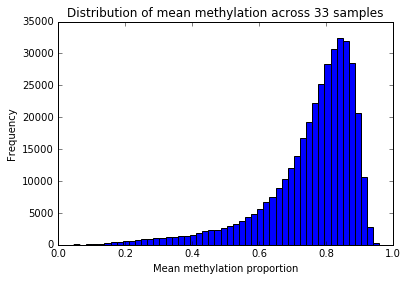
\includegraphics[scale=0.4]{MeanMethylations.png}
\end{minipage}
\end{center}
\end{figure}

\begin{figure}[!ht]
\begin{center}
\caption{Methylation Values across a Single Tissue}
\begin{minipage}[b]{0.40\linewidth}
	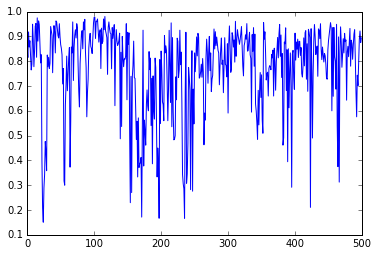
\includegraphics[scale=0.4]{GraphMethylationValues.png}
\end{minipage}
\end{center}
\end{figure}

\subsection{Imputation Pipelines}
The basic structure of our approach remained the same across pipelines. We began by calculating the similarity between the test tissue and the training tissues. The similarity was judged through some type of similarity metric, and different pipelines used different metrics. After measuring similarity, the pipelines combined the information from the most similar tissues to predict the values of the test tissue. The process of combining the information was also varied from pipeline to pipeline.
\subsubsection{Similarity Metrics Tested}
\begin{enumerate}
	\item Beta Distribution Prior Probability
	\item Pearson's R correlation
\end{enumerate}

\subsubsection{Combination Methods Tested}
\begin{enumerate}
	\item Weighted mean
	\item Support Vector Regression
	\item Decision Tree Regression
	\item Random Forest
\end{enumerate}

The pipelines that were run with the beta prior segmented the data into window size chunks, and used those chunks to train the regressors for the given location values.

\subsection{Evaluation}
The effectiveness of each pipeline was judged by examining the Pearson R correlation of the filled in test vector to the full vector, and computing the root mean squared error between the two vectors.

\section{Results}
We tested the pipelines against chromosome 1, and graded the accuracy of the imputation based on the RMSE, and Pearson's R correlation values. The following error rates were achieved by predicting the test sample for chromosome 1. Performance was variable with the weighted mean with correlation similarity performing the best out of all the pipelines.
\begin{center}
	\begin{tabular}{ |p{2cm}|p{2.3cm}|p{2.3cm}|}
		\hline
		\multicolumn{3}{|c|}{\textbf{Imputation Accuracy}} \\
		\hline
		\textbf{Pipeline} & \textbf{RMSE \%} & \textbf{Pearson's R} \\
		\hline
		BPS + SVR & 50.0 & 0.3 \\
		BPS + DT & 17.7  & 0.58 \\
		BPS + RF & 17.7 & 0.58 \\
		CS + WM & 6.3 & 0.93 \\
		\hline
	\end{tabular}
\end{center}

For the weighted mean with correlation similarity pipeline, we optimized how many most similar vectors we looked at in order to impute the test value by graphing the change in the RMSE and the Pearson's R correlation with different top most similar vectors. As figure 5 showcases, the lowest RMSE and the highest correlation occur when 5 columns are considered. For the beta prior similarity pipelines, we segmented the data sets by a given window size, it was predicted that smaller window sizes would perform better because the data would appear more linear on smaller windows, and through trial and error, it was discovered that window size had no effect on the final accuracy.

\begin{figure}[!ht]
\begin{center}
\caption{RMSE and Pearson R change with the number of columns}
\begin{minipage}[b]{0.40\linewidth}
	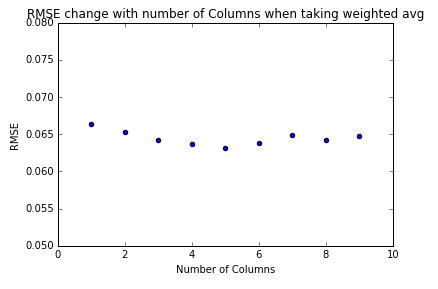
\includegraphics[scale=0.3]{RMSEWeightedMeanOpt.png}
\end{minipage}
\quad
\begin{minipage}[b]{0.40\linewidth}
	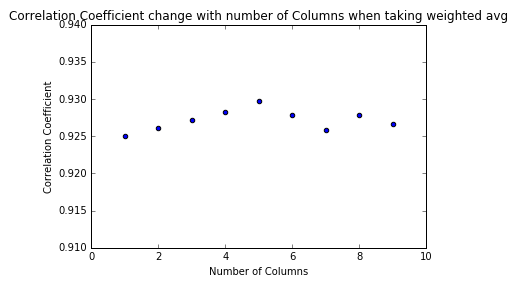
\includegraphics[scale=0.3]{CorrelationWeightedMeanOpt.png}
\end{minipage}
\end{center}
\end{figure}

\section{Discussion and Conclusion}
Once we observed that certain column vectors had strong correlation, we found the top 3 vectors correlated with each tissue and imputed the NANs by taking a weighted mean across the respective chromosome site. The results we obtained using just the simple method of imputing the values of the NANs by using the values at that location in the most highly correlated tissue, which happened to be tissue 23, was already producing better results than the example code that was provided. And as mentioned above, we found the global minimum of RMSE and the global maximum of Correlation Coefficient when we used the top 5 correlated vectors. And this makes sense, because if we use too few columns to compute the average, any chromosome locations that are outliers in the highly correlated tissue could cause a bad prediction, whereas too many columns when used to take the average can introduce noise and superfluous data, especially since not all tissues correlate well.


Thus, when we used 5 columns to take the weighted mean to impute the missing values in the test set, it produced significantly better results. However, we were determined to do even better, and so instead of taking a simple weighted average, we used methods of regression coupled with weighted averaging to try to predict the values. As seen in the data from the previous section, linear regression performed very poorly, but this was expected, because, as mentioned earlier, the data in each column did not follow a linear trend. Polynomial regression performed better than linear, and decision tree regression even more so, but none performed quite as well as taking simply the weighted average itself across the most correlated columns. And this makes sense: regression in this case puts us at a loss of information, because it tries to generalize a tissue to a trend, but we already have a majority of the data in each tissue, since the NANs are so sparse in the training set. Thus, when we regress and predict a value at a chromosome site, we will incur more error than if we were to simply read the data at the row and use the observed value. And so, in this example, in terms of complexity providing better results, we notice that less is more: the easier and more straightforward approach yielded better results, and with good reason.

Similarly, when we tried to use the beta distribution as a prior, we discovered that the vectors that were chosen as the most similar are not as close as the vectors that are chosen with the correlation metric. We believe that this may be part of the reason we see far higher error and lower correlation results for all the pipelines based on beta distribution priors. We hypothesize that the beta priors are not dissimilar enough between different tissues to accurately draw the true closest tissues.

All in all, the weighted mean imputation with the correlation measure used for similarity performed the best. If we had more time, we would try to understand how batch size affects similarity. Perhaps, certain areas of chromosomes are better correlated with other areas of different tissues, rather than looking at a chromosome at the entire tissue level. Breaking down the chromosome into smaller parts may yield more refined results even with just weighted average being used.

\subsubsection*{Acknowledgments}
We would like to acknowledge Princeton University for offering the wonderful COS 424 class that provided us with the opportunity to take on this research. We would also like to thank our Professor, Professor Englehart, and her TA team for providing us with guidance and the tools necessary to make this project happen.

\bibliography{References}
\subsubsection*{References}

\end{document}
